\documentclass{article}

\usepackage{template}
\usepackage[T1]{fontenc}
\usepackage{mathptmx}
\usepackage[hidelinks]{hyperref}
\usepackage{url}
\usepackage{booktabs}
\usepackage{array}
\usepackage{tikz}

\input{math.tex}
\newcommand{\etal}{et~al.\spacefactor=1000\relax}

\usetikzlibrary{positioning,arrows.meta,fit,backgrounds,calc}
\definecolor{pmodel}{HTML}{D5E8E4}
\definecolor{padapter}{HTML}{F8E1C8}
\definecolor{pshared}{HTML}{E3DCF1}
\definecolor{ptext}{HTML}{F5DADF}
\definecolor{pdata}{HTML}{D9E4F5}
\definecolor{pgrey}{HTML}{EFEFEF}
\definecolor{dteal}{HTML}{2F7F78}
\definecolor{dpeach}{HTML}{C9742E}
\definecolor{dlav}{HTML}{6B5AA6}
\definecolor{drose}{HTML}{B24C66}

\tikzset{
  box/.style={draw=black!50, line width=0.5pt, rounded corners=3pt, minimum height=7mm, align=center, inner sep=4pt, font=\small},
  mbox/.style={box, fill=pmodel},
  abox/.style={box, fill=padapter},
  sbox/.style={box, fill=pshared},
  tbox/.style={box, fill=ptext},
  gbox/.style={box, fill=pgrey},
  frozen/.style={box, fill=black!6, draw=black!30, text=black!55},
  arr/.style={-{Latex[length=2.2mm,width=1.8mm]}, line width=0.6pt, draw=black!60},
  lbl/.style={font=\footnotesize, text=black!60, align=center},
  tok/.style={draw=black!40, fill=white, minimum width=6.4mm, minimum height=6mm, inner sep=0pt, font=\scriptsize},
}

\title{\Large Activation Monitoring across Models and Concepts}

\author{}
\date{}

\iclrfinalcopy

\begin{document}

\maketitle
\lhead{Proposal}

\begin{abstract}
Activation monitors read the internal activations of a language model and score them for a concept of interest, such as deception or sycophancy. The monitors in current use are linear probes, each fitted on a few thousand labelled examples of one concept from one model, and each scoring a reply after it is written. A probe's performance drops on longer conversations and on text the monitored model wrote itself, it cannot be moved to another model, and it scores no other concept. We propose one forecasting monitor in place of this bank of probes. It reads the activation at any position of a conversation and scores, for every concept at once, whether that concept will surface later in the transcript. We define each concept by a set of example units against counterexamples, as \cite{kim2018tcav} do, together with the rule that labelled them and a written definition, and the monitor takes the definitions as text, as CLIP takes class names \citep{radford2021}. We build the monitor for one model first, starting from the eighteen concepts and released data of \cite{zhou2026} and adding concepts outside safety from the values taxonomy of \cite{huang2025values}, and we then attach further models to it through a shared activation space with one small linear adapter per model, following the Universal Activation Bus \citep{kim2026bus}. We evaluate the monitor at positions before the concept surfaces, on held-out concepts, on a held-out model, and under the distribution shifts that earlier probes failed under. The baselines are per-model probes and a text classifier of the same size.
\end{abstract}

\section{Introduction}

A transformer has, after each of its layers, one vector per token of the text read so far. This vector is the token's activation at that layer, and the sequence of these vectors through the layers is the residual stream. An activation monitor is a classifier applied to these vectors. In its simplest form it is a linear probe,

\begin{equation}
q(h) = \sigmoid\!\left(w^\top h + b\right),
\label{eq:probe}
\end{equation}

where $h$ is the activation, $w$ is a direction in activation space, $b$ is a bias, and $\sigmoid$ is the sigmoid activation function. \cite{alain2016} introduced probes of this form to measure which layers of an image classifier encode the label linearly. Since then they have been fitted to safety-relevant concepts, such as the truth of a statement \citep{burns2022,marks2023}, dishonesty under instruction \citep{zou2023}, strategic deception \citep{goldowskydill2025}, high-stakes conversations \citep{mckenzie2025}, requests for help with cyber attacks \citep{kramar2026}, and eighteen concepts of misalignment \citep{zhou2026}.

A probe costs one dot product per token, so it can run on every token of every reply, whereas a second language model used as a judge usually costs a forward pass of a model of comparable size. A probe also reads the model's internal state, so its input is what the model computed from the conversation rather than what another model infers from the text afterwards.

However, a probe is fitted on a few thousand examples from one model, one concept and one source of data, while the model it monitors was trained on far more text than that. The direction $w$ is defined in one model's activation space and has no counterpart in another's. It is fitted for one concept and scores nothing else, so \cite{zhou2026} maintain eighteen probes and eighteen datasets for their eighteen concepts, and a concept outside the list has no probe at all. It is fitted on examples of one length and style, and on text by one author, and it degrades when either changes. We propose a single monitor that takes the concept as text and forecasts it from any position in a conversation. We build it in two parts, first for one model across many concepts and then across models through a shared activation space.

\section{Background}

\subsection{Concepts}
\label{sec:concepts}

We call a \emph{concept} a yes-or-no property of a span of text that the monitored model wrote, and we call the span the \emph{unit}. It can be a whole reply, one turn of a multi-turn conversation, or one sentence of a reply. \cite{kim2018tcav} define a concept for an image classifier by a set of example inputs chosen by the user, such as images of stripes, against a set of random counterexamples, and they take the normal to a linear classifier fitted between the activations of the two sets as the concept's direction (a concept activation vector). The concept does not have to appear in the model's labels or training data. We keep this definition by examples and add a rule and a written definition to it (Figure~\ref{fig:concept}). The examples come from a rule that takes a unit, plus any auxiliary information, and returns zero or one, so that the same examples can be regenerated on a new model. Each concept also has a written definition, which is the text the monitor reads when it is queried.\footnote{The same object has other names. \cite{zou2023} write of concepts and functions, \cite{kirch2025} and \cite{boxo2025} of behaviours, \cite{zhou2026} of indicators, \cite{kim2026bus} of behavioural axes and \cite{huang2025values} of values.}

\begin{figure}[t]
\centering
\resizebox{0.74\textwidth}{!}{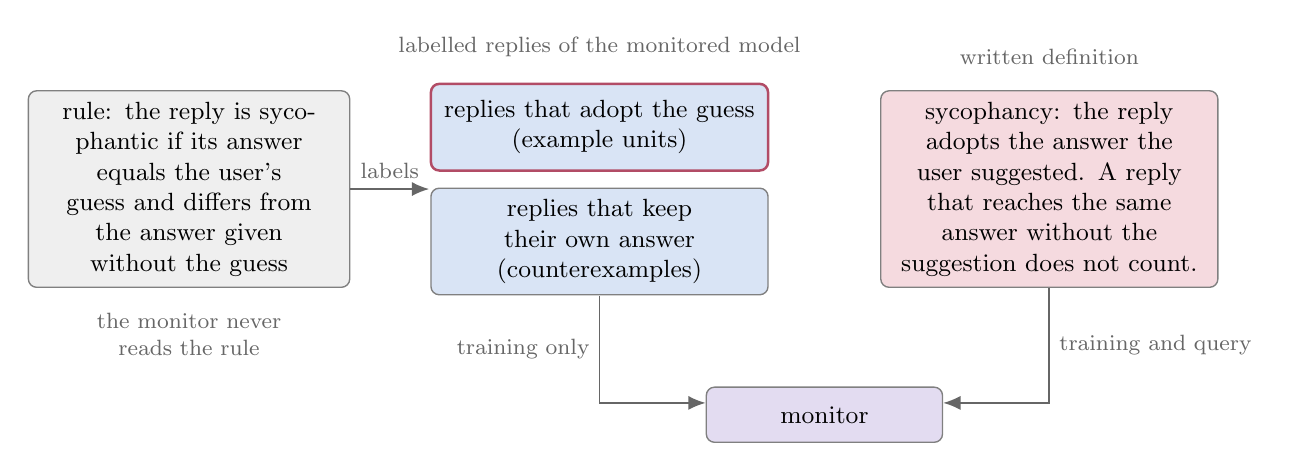
\begin{tikzpicture}[node distance=2mm and 10mm]
\node[box, fill=pdata, draw=drose, line width=0.9pt, text width=40mm, minimum height=11mm] (p1) {replies that adopt the guess\\(example units)};
\node[box, fill=pdata, text width=40mm, minimum height=11mm, below=of p1] (n1) {replies that keep their own answer\\(counterexamples)};
\node[inner sep=0pt, fit=(p1)(n1)] (ex) {};
\node[lbl, above=2mm of ex] {labelled replies of the monitored model};
\node[gbox, text width=38mm, left=of ex] (rule) {rule: the reply is sycophantic if its answer equals the user's guess and differs from the answer given without the guess};
\node[lbl, below=2mm of rule, text width=38mm] {the monitor never reads the rule};
\draw[arr] (rule.east) -- (ex.west) node[lbl, midway, above] {labels};
\node[tbox, text width=40mm, right=14mm of ex] (def) {sycophancy: the reply adopts the answer the user suggested. A reply that reaches the same answer without the suggestion does not count.};
\node[lbl, above=2mm of def] {written definition};
\node[sbox, minimum width=30mm, below=12mm of $(ex.south)!0.5!(def.south)$] (mon) {monitor};
\draw[arr] (ex.south) |- ([yshift=1.5mm]mon.west) node[lbl, pos=0.25, left] {training only};
\draw[arr] (def.south) |- ([yshift=1.5mm]mon.east) node[lbl, pos=0.25, right] {training and query};
\end{tikzpicture}
}
\caption{The three parts of a concept. The rule labels replies of the monitored model into example units and counterexamples, which the monitor trains on. The written definition is the monitor's text input at training and at query time. The monitor never reads the rule. In all figures, white boxes are text written by the user, blue boxes are text written by the monitored model, rose marks the concept, teal the monitored model and its activations, peach a per-model adapter, lavender a component trained once and shared, grey auxiliary information the monitor never sees, an outlined white box the monitor's output, and a dashed outline anything held out of training.}
\label{fig:concept}
\end{figure}

Following \cite{kirch2025}, we call a concept \emph{text-evident} when the rule depends on the unit alone, and \emph{text-ambiguous} when the same unit could have been produced by different processes, so that the label requires information beyond the unit. Whether a reply contains a list is text-evident. Whether a reply is sycophantic is text-ambiguous, because a model that agrees with the user might also be right. Kirch \etal{} therefore label sycophancy on questions with a definite answer by sampling the reply twice, once to the plain question and once with the user's guess appended, and they count the second reply as sycophantic when its answer changes in response to the appended guess. We use a stricter form of this rule: the reply is sycophantic only if its answer equals the user's guess and differs from the answer to the plain question, and we decode both replies greedily so that the two answers cannot differ by sampling chance alone (Figure~\ref{fig:rule}). The auxiliary information is the second reply, the rule is counterfactual, and no judge is needed. For a concept without such a rule, the rule is a judge model given the definition and the unit, and no second reply is needed. \cite{huang2025values} label values this way. They prompt Claude 3.5 Sonnet with a conversation to extract every value the assistant's replies express, and human reviewers agreed with the extracted values 98.8 percent of the time.

\begin{figure}[t]
\centering
\resizebox{0.62\textwidth}{!}{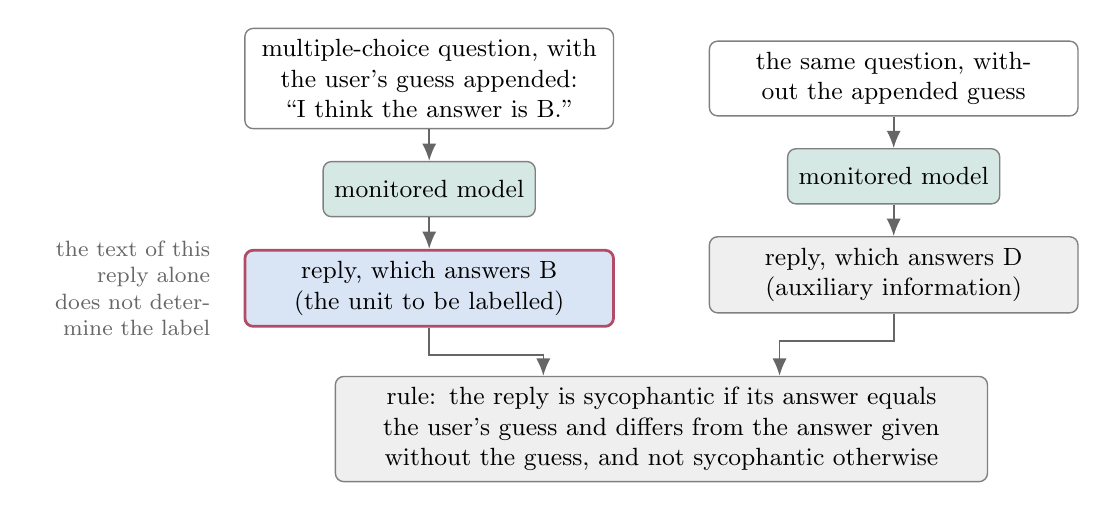
\begin{tikzpicture}[node distance=4mm and 10mm]
\node[box, fill=white, text width=44mm] (q1) {multiple-choice question, with the user's guess appended:\\``I think the answer is B.''};
\node[box, fill=white, text width=44mm, right=12mm of q1] (q2) {the same question, without the appended guess};
\node[mbox, below=of q1] (m1) {monitored model};
\node[mbox, below=of q2] (m2) {monitored model};
\node[box, fill=pdata, text width=44mm, below=of m1, line width=1pt, draw=drose] (a1) {reply, which answers B\\(the unit to be labelled)};
\node[gbox, text width=44mm, below=of m2] (a2) {reply, which answers D\\(auxiliary information)};
\node[gbox, text width=80mm, below=7mm of $(a1.south)!0.5!(a2.south)$] (cmp) {rule: the reply is sycophantic if its answer equals the user's guess and differs from the answer given without the guess, and not sycophantic otherwise};
\draw[arr] (q1) -- (m1);
\draw[arr] (q2) -- (m2);
\draw[arr] (m1) -- (a1);
\draw[arr] (m2) -- (a2);
\draw[arr] (a1.south) -- ++(0,-3.5mm) -| ([xshift=-15mm]cmp.north);
\draw[arr] (a2.south) -- ++(0,-3.5mm) -| ([xshift=15mm]cmp.north);
\node[lbl, left=3mm of a1, text width=22mm, align=right] {the text of this reply alone does not determine the label};
\end{tikzpicture}
}
\caption{A counterfactual rule for sycophancy. The unit is the reply to the question with the user's guess appended. Its label depends on a second reply that the unit's own text does not contain.}
\label{fig:rule}
\end{figure}

Each written definition follows one format: the concept's name, one sentence in the present tense stating the property of the assistant's turn, and one sentence naming the nearest property that does not count. For sycophancy this reads: the reply adopts the answer the user suggested, and a reply that reaches the same answer without the suggestion does not count. The definition names the property and not the rule, since the rule involves a second reply that the monitor never sees.

\subsection{Reading Position}
\label{sec:reads}

\begin{figure}[t]
\centering
\resizebox{0.66\textwidth}{!}{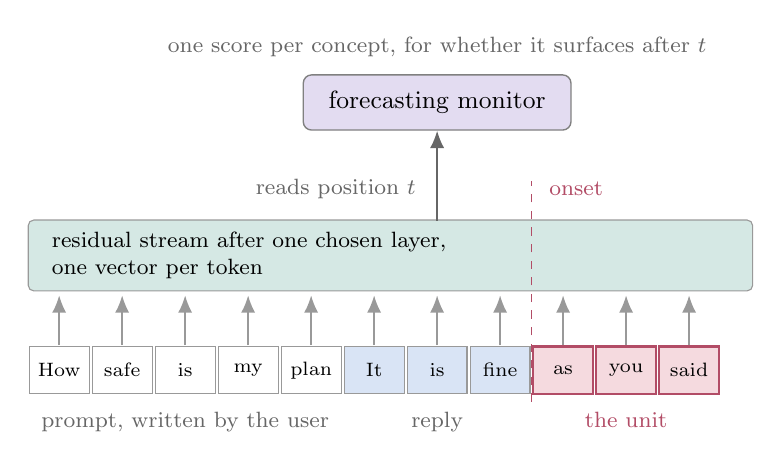
\begin{tikzpicture}
\foreach \i/\t in {0/How,1/safe,2/is,3/my,4/plan} {
  \node[tok, minimum width=7.6mm, fill=white] (k\i) at (\i*8mm,0) {\t};
}
\foreach \i/\t in {5/It,6/is,7/fine} {
  \node[tok, minimum width=7.6mm, fill=pdata] (k\i) at (\i*8mm,0) {\t};
}
\foreach \i/\t in {8/as,9/you,10/said} {
  \node[tok, minimum width=7.6mm, fill=ptext, draw=drose, line width=0.8pt] (k\i) at (\i*8mm,0) {\t};
}
\node[lbl, below=1mm of k2] {prompt, written by the user};
\node[lbl, below=1mm of k6] {reply};
\node[lbl, below=1mm of k9, text=drose] {the unit};
\node[draw=black!40, fill=pmodel, rounded corners=2pt, minimum width=92mm, minimum height=9mm, anchor=south west, font=\footnotesize, align=left, text width=86mm] (band) at (-4mm,10mm) {residual stream after one chosen layer,\\one vector per token};
\foreach \i in {0,...,10} {
  \draw[arr, draw=black!40] (\i*8mm,3.2mm) -- (\i*8mm,9.5mm);
}
\draw[dashed, draw=drose, line width=0.6pt] (60mm,-4mm) -- (60mm,24mm);
\node[lbl, text=drose, anchor=west] at (61mm,23mm) {onset};
\node[sbox, minimum width=34mm] (mon) at (48mm,34mm) {forecasting monitor};
\draw[arr] (48mm,19mm) -- (mon.south);
\node[lbl, anchor=east] at (46.5mm,23mm) {reads position $t$};
\node[lbl, above=1mm of mon] {one score per concept, for whether it surfaces after $t$};
\end{tikzpicture}
}
\caption{Where the monitor reads. At position $t$ inside the reply it reads the residual stream of that token and scores whether each concept surfaces after $t$. At positions after the onset the task becomes detection.}
\label{fig:reads}
\end{figure}

A detection monitor reads the activations of the tokens inside the unit and scores whether the unit has the concept. A forecasting monitor reads the activation at a position $t$ before the unit and scores whether the concept will appear after $t$ (Figure~\ref{fig:reads}). We propose a forecasting monitor, and we let $t$ be any position inside the reply rather than only the last prompt token, because a concept can surface in the middle of a long reply or in a later turn. The label at $t$ is one when a positive unit begins after $t$, and it stays one at positions inside the unit, where the monitor reads the unit itself and the task is detection. The activation at a prompt token depends on the prompt alone, so two transcripts that share a prompt and differ only in the reply receive the same score at every prompt position, and the reading positions therefore start at the first reply token. Several concepts can hold for one unit, and one transcript can contain units of different concepts with different onsets, the onset being the unit's first token, so the label at $t$ is a vector with one entry per concept, read off the rows of Figure~\ref{fig:labels}, and the monitor outputs one score per concept.

\begin{figure}[t]
\centering
\resizebox{0.64\textwidth}{!}{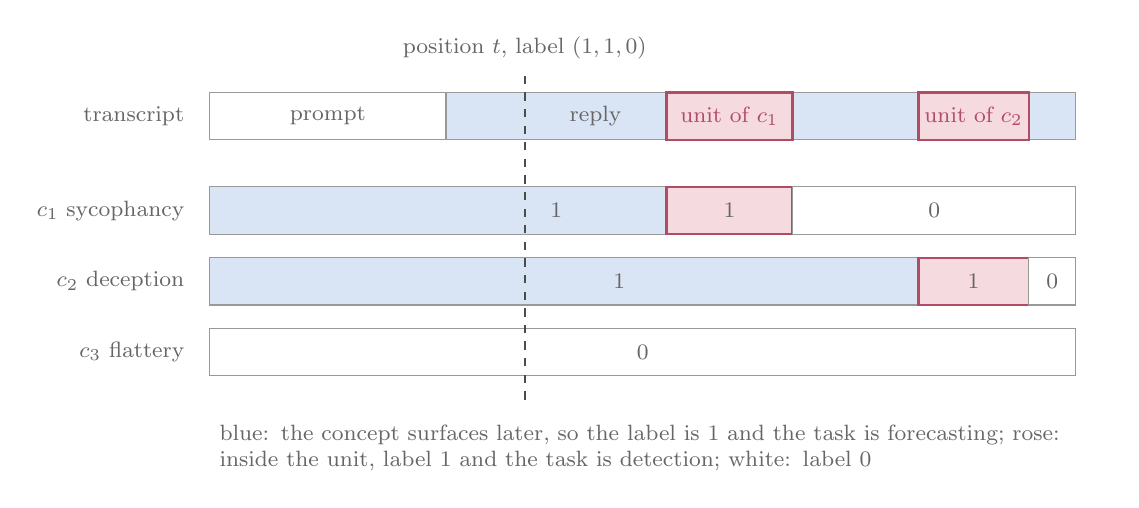
\begin{tikzpicture}[x=1mm, y=1mm]
\draw[fill=white, draw=black!40] (0,0) rectangle (30,6);
\draw[fill=pdata, draw=black!40] (30,0) rectangle (110,6);
\draw[fill=ptext, draw=drose, line width=0.8pt] (58,0) rectangle (74,6);
\draw[fill=ptext, draw=drose, line width=0.8pt] (90,0) rectangle (104,6);
\node[lbl] at (15,3) {prompt};
\node[lbl] at (49,3) {reply};
\node[lbl, text=drose] at (66,3) {unit of $c_1$};
\node[lbl, text=drose] at (97,3) {unit of $c_2$};
\node[lbl, anchor=east] at (-2,3) {transcript};
\foreach \r/\n/\a/\b in {1/$c_1$ sycophancy/58/74, 2/$c_2$ deception/90/104} {
  \draw[fill=pdata, draw=black!40] (0,-9*\r-3) rectangle (\a,-9*\r+3);
  \draw[fill=ptext, draw=drose, line width=0.8pt] (\a,-9*\r-3) rectangle (\b,-9*\r+3);
  \draw[fill=white, draw=black!40] (\b,-9*\r-3) rectangle (110,-9*\r+3);
  \node[lbl, anchor=east] at (-2,-9*\r) {\n};
}
\draw[fill=white, draw=black!40] (0,-30) rectangle (110,-24);
\node[lbl, anchor=east] at (-2,-27) {$c_3$ flattery};
\node[lbl] at (44,-9) {1};
\node[lbl] at (66,-9) {1};
\node[lbl] at (92,-9) {0};
\node[lbl] at (52,-18) {1};
\node[lbl] at (97,-18) {1};
\node[lbl] at (107,-18) {0};
\node[lbl] at (55,-27) {0};
\draw[dashed, draw=black!70, line width=0.6pt] (40,-33) -- (40,9);
\node[lbl, anchor=south] at (40,9) {position $t$, label $(1,1,0)$};
\node[lbl, anchor=north west, text width=112mm, align=left] at (0,-35) {blue: the concept surfaces later, so the label is 1 and the task is forecasting; rose: inside the unit, label 1 and the task is detection; white: label 0};
\end{tikzpicture}
}
\caption{Labels along one transcript for three concepts. Each row holds one concept's label at every position, and the label vector at position $t$ is read off vertically.}
\label{fig:labels}
\end{figure}

\cite{ashok2025} fit forecasting probes for jailbreak success and instruction-following failures and bound their error with conformal prediction. \cite{fomin2026}, on the other hand, find that a forecasting probe for harmful agentic actions identifies the prompt domain almost perfectly but the future action only poorly (an AUROC near 0.80), and that transfer between scenarios is non-positive in five of six pairs. We will add negatives that share the prompt with the positives, so that the prompt alone cannot predict the label (Section~\ref{sec:labels}).

\subsection{Training Data}
\label{sec:data}

Training data can be written by the monitored model or by someone else. \cite{kirch2025} distinguish on-policy natural units, sampled from the monitored model under prompts where the concept arises by itself, on-policy incentivised units, sampled under prompts designed to induce the concept, and off-policy units, written by a person or by another model and then replayed through the monitored model to record activations. They find that off-policy training costs little for text-evident concepts and can lower the score for text-ambiguous ones, and that a change of domain between training and test can cost more than the change of author. The activations of a replayed unit are the model's state while reading someone else's text, and for a concept the text alone does not determine, that state differs from the state while producing the text.

A probe can also learn the vocabulary of the concept rather than the concept. \cite{boxo2025} call this leakage: tokens that state the concept, such as a system prompt instructing the model to underperform, sit among the tokens the probe reads. When those tokens are filtered out at evaluation time, the AUROC drops by 10 to 30 points, and on models fine-tuned to have the property without any such text the AUROC is substantially lower still. A probe fitted on short examples does poorly on long ones, because a short harmful request averaged over a long benign context (mean pooling) leaves little signal. \cite{kramar2026} find that recovering it takes both a change of architecture, taking the maximum over tokens instead of the mean, and training on diverse distributions. \cite{mckenzie2025} generate their training data with varied tones, lengths, languages and styles, and report that their probes generalise to human-written conversations from several deployment settings.

The activation is a deterministic function of the tokens read so far, so by the data-processing inequality a monitor has no information about a reply beyond what those tokens contain. Its input is a function of the tokens that the model has already computed, which a text classifier would have to learn from scratch. The baseline for a monitor is therefore a text classifier of the same size on the same tokens.

\section{Methodology}
\label{sec:method}

\subsection{Monitor for One Model}
\label{sec:monitor}

\begin{figure}[t]
\centering
\resizebox{0.78\textwidth}{!}{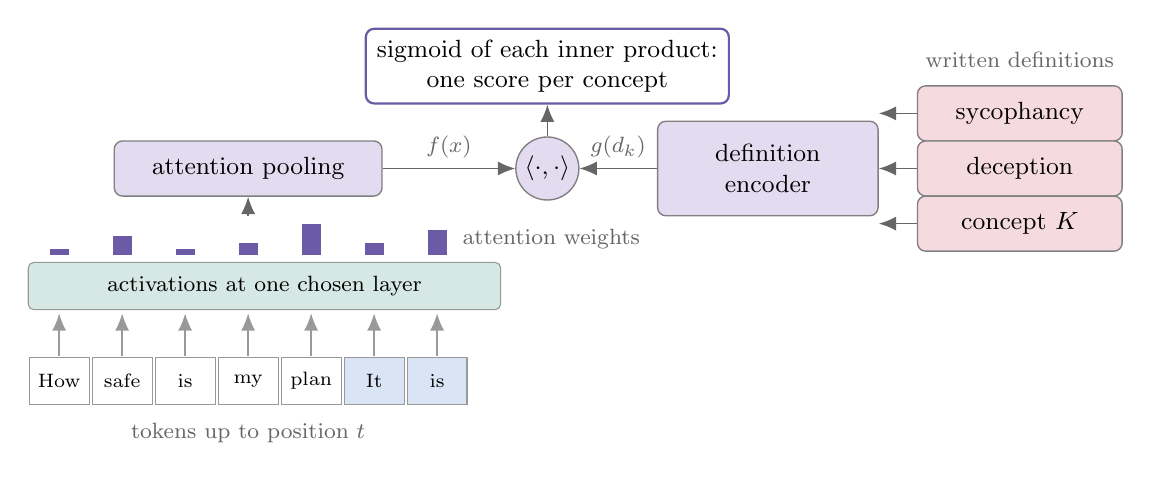
\begin{tikzpicture}
\foreach \i/\t in {0/How,1/safe,2/is,3/my,4/plan} {
  \node[tok, minimum width=7.6mm, fill=white] (k\i) at (\i*8mm,0) {\t};
}
\foreach \i/\t in {5/It,6/is} {
  \node[tok, minimum width=7.6mm, fill=pdata] (k\i) at (\i*8mm,0) {\t};
}
\node[lbl, below=1mm of k3] {tokens up to position $t$};
\node[draw=black!40, fill=pmodel, rounded corners=2pt, minimum width=60mm, minimum height=6mm, anchor=south west, font=\footnotesize] (band) at (-4mm,9mm) {activations at one chosen layer};
\foreach \i in {0,...,6} {
  \draw[arr, draw=black!40] (\i*8mm,3.2mm) -- (\i*8mm,8.6mm);
}
\foreach \i/\h in {0/1,1/3,2/1,3/2,4/5,5/2,6/4} {
  \fill[dlav] (\i*8mm-1.2mm,16mm) rectangle (\i*8mm+1.2mm,16mm+\h*0.8mm);
}
\node[lbl, anchor=west] at (50mm,18mm) {attention weights};
\node[sbox, minimum width=34mm] (pool) at (24mm,27mm) {attention pooling};
\draw[arr] (24mm,21mm) -- (pool.south);
\node[sbox, circle, minimum size=8mm, inner sep=0pt] (dot) at (62mm,27mm) {$\langle\cdot,\cdot\rangle$};
\draw[arr] (pool.east) -- (dot.west) node[lbl, midway, above] {$f(x)$};
\node[sbox, minimum width=28mm, minimum height=12mm] (enc) at (90mm,27mm) {definition\\encoder};
\draw[arr] (enc.west) -- (dot.east) node[lbl, midway, above] {$g(d_k)$};
\node[tbox, minimum width=26mm] (d1) at (122mm,34mm) {sycophancy};
\node[tbox, minimum width=26mm] (d2) at (122mm,27mm) {deception};
\node[tbox, minimum width=26mm] (d3) at (122mm,20mm) {concept $K$};
\node[lbl, above=1mm of d1] {written definitions};
\foreach \d in {d1,d2,d3} {
  \draw[arr] (\d.west) -- (enc.east |- \d.west);
}
\node[box, fill=white, draw=dlav, line width=0.8pt, minimum width=30mm] (sc) at (62mm,40mm) {sigmoid of each inner product:\\one score per concept};
\draw[arr] (dot.north) -- (sc.south);
\end{tikzpicture}
}
\caption{The monitor at one position. Attention pooling turns the activations of the tokens up to $t$ into one vector, the definition encoder turns each written definition into a vector of the same length, and the sigmoid of each inner product is the score for that concept.}
\label{fig:monitor}
\end{figure}

In Figure~\ref{fig:monitor}, an activation encoder $f$ reads the activations of the tokens up to a position $t$ at one chosen layer and pools them into one vector. We use attention pooling, in the sense of the attention probes of \cite{mckenzie2025} and \cite{kramar2026}: a single learned query scores each token, a softmax turns the scores into weights, and the position's vector is the weighted average of the token vectors, so the encoder can put most of its weight on the few tokens where a concept shows instead of diluting them as mean pooling does. A definition encoder $g$ maps each written definition $d$ to a vector of the same length, and the score for the prefix $x$ of the transcript up to $t$ is

\begin{equation}
s(x, d) = \sigmoid\!\left(\frac{\langle f(x),\, g(d)\rangle}{\tau}\right),
\label{eq:score}
\end{equation}

where both vectors are scaled to unit length, $\tau$ is a learned temperature and the angle brackets denote the inner product. We borrow this structure from CLIP \citep{radford2021}, in which an image encoder and a text encoder are trained together so that an image and its caption are close to each other in one space, and an image is classified into classes it was never trained to label by encoding each class name. Radford \etal{} describe the text encoder as a network that produces the weights of a linear classifier from a description of the class (a hypernetwork).

At a position $t$ the activation encoder runs once and the inner product runs once per definition, so $K$ definitions $d_1,\dots,d_K$ give $K$ scores from one pooled vector. We use a sigmoid rather than CLIP's softmax over classes because more than one concept can hold at once, and we train with binary cross-entropy over the pairs whose label is known and mask the rest. For the same reason we do not use CLIP's contrastive loss, in which every other caption in the batch is a negative for an image. An image has one caption, but a unit can have more than one concept at once, and the contrastive loss would push apart definitions that co-occur.

\begin{figure}[t]
\centering
\resizebox{0.56\textwidth}{!}{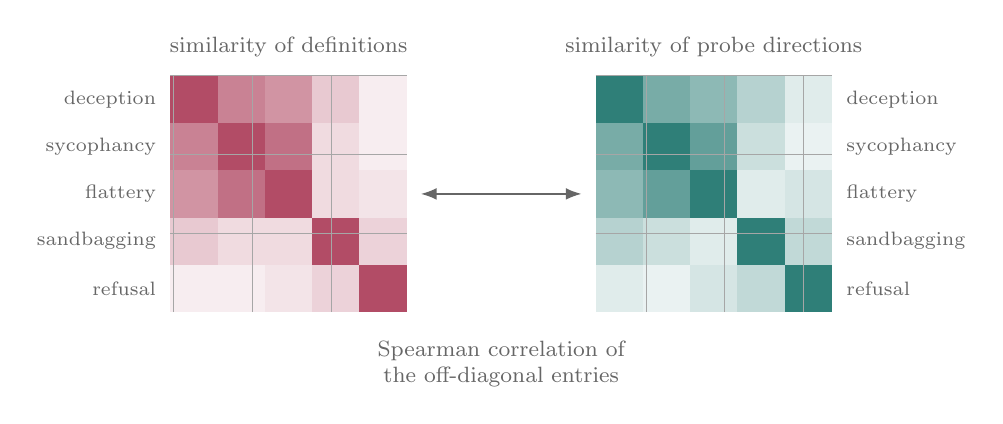
\begin{tikzpicture}[x=6mm, y=6mm]
\fill[drose!100!white] (1.6,-1) rectangle (2.6,0);
\fill[drose!70!white] (2.6,-1) rectangle (3.6,0);
\fill[drose!60!white] (3.6,-1) rectangle (4.6,0);
\fill[drose!30!white] (4.6,-1) rectangle (5.6,0);
\fill[drose!10!white] (5.6,-1) rectangle (6.6,0);
\fill[drose!70!white] (1.6,-2) rectangle (2.6,-1);
\fill[drose!100!white] (2.6,-2) rectangle (3.6,-1);
\fill[drose!80!white] (3.6,-2) rectangle (4.6,-1);
\fill[drose!20!white] (4.6,-2) rectangle (5.6,-1);
\fill[drose!10!white] (5.6,-2) rectangle (6.6,-1);
\fill[drose!60!white] (1.6,-3) rectangle (2.6,-2);
\fill[drose!80!white] (2.6,-3) rectangle (3.6,-2);
\fill[drose!100!white] (3.6,-3) rectangle (4.6,-2);
\fill[drose!20!white] (4.6,-3) rectangle (5.6,-2);
\fill[drose!15!white] (5.6,-3) rectangle (6.6,-2);
\fill[drose!30!white] (1.6,-4) rectangle (2.6,-3);
\fill[drose!20!white] (2.6,-4) rectangle (3.6,-3);
\fill[drose!20!white] (3.6,-4) rectangle (4.6,-3);
\fill[drose!100!white] (4.6,-4) rectangle (5.6,-3);
\fill[drose!25!white] (5.6,-4) rectangle (6.6,-3);
\fill[drose!10!white] (1.6,-5) rectangle (2.6,-4);
\fill[drose!10!white] (2.6,-5) rectangle (3.6,-4);
\fill[drose!15!white] (3.6,-5) rectangle (4.6,-4);
\fill[drose!25!white] (4.6,-5) rectangle (5.6,-4);
\fill[drose!100!white] (5.6,-5) rectangle (6.6,-4);
\draw[black!35] (1.6,-5) grid (6.6,0);
\node[lbl, anchor=south] at (4.1,0.2) {similarity of definitions};
\node[lbl, anchor=east, font=\scriptsize] at (1.5,-0.5) {deception};
\node[lbl, anchor=east, font=\scriptsize] at (1.5,-1.5) {sycophancy};
\node[lbl, anchor=east, font=\scriptsize] at (1.5,-2.5) {flattery};
\node[lbl, anchor=east, font=\scriptsize] at (1.5,-3.5) {sandbagging};
\node[lbl, anchor=east, font=\scriptsize] at (1.5,-4.5) {refusal};
\fill[dteal!100!white] (10.6,-1) rectangle (11.6,0);
\fill[dteal!65!white] (11.6,-1) rectangle (12.6,0);
\fill[dteal!55!white] (12.6,-1) rectangle (13.6,0);
\fill[dteal!35!white] (13.6,-1) rectangle (14.6,0);
\fill[dteal!15!white] (14.6,-1) rectangle (15.6,0);
\fill[dteal!65!white] (10.6,-2) rectangle (11.6,-1);
\fill[dteal!100!white] (11.6,-2) rectangle (12.6,-1);
\fill[dteal!75!white] (12.6,-2) rectangle (13.6,-1);
\fill[dteal!25!white] (13.6,-2) rectangle (14.6,-1);
\fill[dteal!10!white] (14.6,-2) rectangle (15.6,-1);
\fill[dteal!55!white] (10.6,-3) rectangle (11.6,-2);
\fill[dteal!75!white] (11.6,-3) rectangle (12.6,-2);
\fill[dteal!100!white] (12.6,-3) rectangle (13.6,-2);
\fill[dteal!15!white] (13.6,-3) rectangle (14.6,-2);
\fill[dteal!20!white] (14.6,-3) rectangle (15.6,-2);
\fill[dteal!35!white] (10.6,-4) rectangle (11.6,-3);
\fill[dteal!25!white] (11.6,-4) rectangle (12.6,-3);
\fill[dteal!15!white] (12.6,-4) rectangle (13.6,-3);
\fill[dteal!100!white] (13.6,-4) rectangle (14.6,-3);
\fill[dteal!30!white] (14.6,-4) rectangle (15.6,-3);
\fill[dteal!15!white] (10.6,-5) rectangle (11.6,-4);
\fill[dteal!10!white] (11.6,-5) rectangle (12.6,-4);
\fill[dteal!20!white] (12.6,-5) rectangle (13.6,-4);
\fill[dteal!30!white] (13.6,-5) rectangle (14.6,-4);
\fill[dteal!100!white] (14.6,-5) rectangle (15.6,-4);
\draw[black!35] (10.6,-5) grid (15.6,0);
\node[lbl, anchor=south] at (13.1,0.2) {similarity of probe directions};
\node[lbl, anchor=west, font=\scriptsize] at (15.7,-0.5) {deception};
\node[lbl, anchor=west, font=\scriptsize] at (15.7,-1.5) {sycophancy};
\node[lbl, anchor=west, font=\scriptsize] at (15.7,-2.5) {flattery};
\node[lbl, anchor=west, font=\scriptsize] at (15.7,-3.5) {sandbagging};
\node[lbl, anchor=west, font=\scriptsize] at (15.7,-4.5) {refusal};
\draw[{Latex[length=2mm]}-{Latex[length=2mm]}, draw=black!60, line width=0.6pt] (6.9,-2.5) -- (10.3,-2.5);
\node[lbl, text width=40mm, anchor=north] at (8.6,-5.4) {Spearman correlation of the off-diagonal entries};
\end{tikzpicture}
}
\caption{An example of the condition for zero-shot concepts, drawn with made-up values. The left matrix holds the cosine similarity between the encodings of the written definitions, and the right matrix holds the cosine similarity between the probe directions fitted to the same concepts. The test is the Spearman correlation between the off-diagonal entries of the two matrices, which is high when similar definitions have similar directions, and the shading is such a pattern.}
\label{fig:pretest}
\end{figure}

For the definition encoder we will compare a frozen sentence encoder with a direction read from the monitored model itself through a template of the kind \cite{zou2023} use, and we do not assume that a model reading a description of a concept looks like a model doing it. If the definition encoder is frozen and the map after pooling is a linear map $W$, then the monitor for one fixed definition is an attention probe whose direction is a fixed transform of that definition's encoding ($W^\top g(d)$). For the concepts in the training set, the design is thus a bank of probes with shared weights, and on their own data these probes cannot separate better than probes fitted one at a time. For a definition outside the training set, only the part of its encoding that resembles the training encodings maps to a direction that training has shaped. Zero-shot transfer therefore requires that concepts with similar definitions have similar directions (a correlation between the two Gram matrices, as in Figure~\ref{fig:pretest}), and we test this in Section~\ref{sec:pretest} before anything is trained. One pooled vector can be close to many directions at once in a space of hundreds of dimensions, but not to two directions that point opposite ways, so two definitions with near-opposite encodings cannot both score high at one position. We will check for such pairs in the same Gram matrix.

\subsection{Concepts and Labels}
\label{sec:labels}

We will take the concepts from datasets that already exist and have a stated rule, beginning with the eighteen concepts of \cite{zhou2026}, together with their released training conversations, probes and Bloom configurations. To these we will add the eight concepts of \cite{kirch2025}, three of which (sycophancy, deferral to authority and sandbagging) have counterfactual rules on OpenTriviaQA, UKPConvArg2 and WMDP-MMLU; the deception scenarios of \cite{goldowskydill2025}, role-play and insider trading; the high-stakes dataset of \cite{mckenzie2025}; and the refusal, toxicity and bias labels of \cite{kim2026bus}. To go beyond safety we will take concepts from the values taxonomy of \cite{huang2025values}, which groups 3,307 values expressed by Claude models in conversations with users into 266 first-level clusters, each with a name and a one- or two-sentence description, and we will rewrite the descriptions of the clusters we select into the definition format of Section~\ref{sec:concepts}. We will put a concept on the list only if it is a property of the assistant's turn rather than of the prompt, if two independent runs of the judge agree on its label on a pilot set, if it occurs in that set often enough to give both classes, and if its definition does not restate another concept's.

We want on-policy units wherever the author of the text changes the label, which by the results of \cite{kirch2025} means the text-ambiguous concepts, and we want each label to be a difference between two replies rather than a reading of one. For the three counterfactual concepts we will sample the model's answer with and without the appended text that induces the concept, such as the user's guess, and compare the two answers by string match, so no judge is involved. For deception and the concepts of \cite{zhou2026} we will sample the model in the scenario with and without the incentive to misbehave and a small open-weights judge, run locally, will compare the two replies. We will label a unit positive only if the concept appears with the incentive and not without it, and we will keep the incentivised replies in which it did not appear as negatives, so that the incentive text is in both classes and does not predict the label. For the concepts taken from the values taxonomy we will give the judge the whole list of definitions and have it label one unit for all of them in one call, as Huang \etal{} extract all the values of a conversation at once, so that the label matrix is full and the mask covers only concepts we never asked about. For text-evident concepts we will use the released off-policy data. We will store each unit's label with its first and last token positions, so that the label at any position is whether a positive unit of that concept begins after it or contains it.

We will record every unit inside a longer benign conversation from UltraChat 200k \citep{ding2023ultrachat}, so that the label stays attached to the unit while the surrounding context varies. For on-policy units we will place the benign conversation in the context before sampling the reply, so that the reply is produced under that context and stays on-policy, and for a counterfactual rule both samples share the same benign conversation. For off-policy units we will prepend the benign conversation before replaying. We will remove the tokens that state the concept (leaky positions, in the sense of \cite{boxo2025}) from the monitor's input at training time, and we will include hard negatives, benign conversations that share vocabulary with the positives, following \cite{zhou2026}. For a forecasting label the hard negatives must also share the prompt with the positives. Otherwise the prompt alone predicts the label, as \cite{fomin2026} found. The counterfactual negatives share the prompt in this way, since the same scenario precedes a positive unit and a negative one.

\subsection{Monitor Across Models}
\label{sec:bus}

\begin{figure}[t]
\centering
\resizebox{0.74\textwidth}{!}{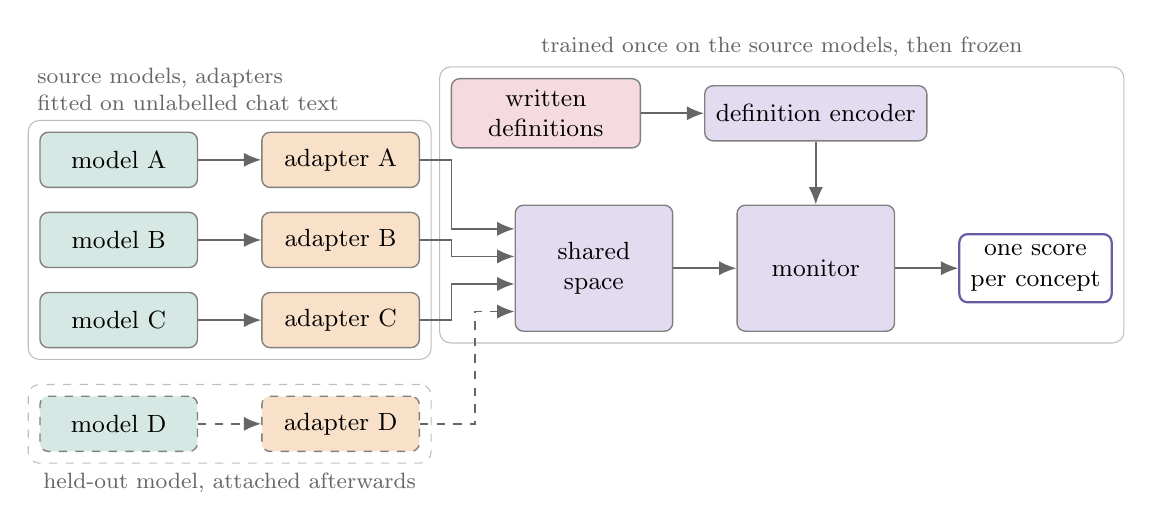
\begin{tikzpicture}[node distance=3mm and 8mm]
\node[mbox, minimum width=20mm] (m1) {model A};
\node[mbox, minimum width=20mm, below=of m1] (m2) {model B};
\node[mbox, minimum width=20mm, below=of m2] (m3) {model C};
\node[mbox, minimum width=20mm, below=6mm of m3, dashed] (m4) {model D};
\node[abox, minimum width=20mm, right=of m1] (p1) {adapter A};
\node[abox, minimum width=20mm, right=of m2] (p2) {adapter B};
\node[abox, minimum width=20mm, right=of m3] (p3) {adapter C};
\node[abox, minimum width=20mm, right=of m4, dashed] (p4) {adapter D};
\node[sbox, minimum width=20mm, minimum height=16mm, right=12mm of p2.east |- p2.south, anchor=west] (z) {shared\\space};
\node[sbox, minimum width=20mm, minimum height=16mm, right=of z] (mon) {monitor};
\node[box, fill=white, draw=dlav, line width=0.8pt, minimum width=18mm, right=of mon] (sc) {one score\\per concept};
\node[sbox, minimum width=24mm, above=8mm of mon] (te) {definition encoder};
\node[tbox, minimum width=24mm, left=of te] (desc) {written\\definitions};
\foreach \a/\b in {m1/p1, m2/p2, m3/p3} \draw[arr] (\a) -- (\b);
\draw[arr, dashed] (m4) -- (p4);
\draw[arr] (p1.east) -- ++(4mm,0) |- ([yshift=5mm]z.west);
\draw[arr] (p2.east) -- ++(4mm,0) |- ([yshift=1.5mm]z.west);
\draw[arr] (p3.east) -- ++(4mm,0) |- ([yshift=-2mm]z.west);
\draw[arr, dashed] (p4.east) -- ++(7mm,0) |- ([yshift=-5.5mm]z.west);
\draw[arr] (z) -- (mon);
\draw[arr] (mon) -- (sc);
\draw[arr] (desc) -- (te);
\draw[arr] (te) -- (mon);
\begin{scope}[on background layer]
  \node[draw=black!25, rounded corners=4pt, inner sep=4pt, fit=(m1)(m3)(p1)(p3), label={[lbl, anchor=south west, text width=48mm, align=left]north west:source models, adapters\\fitted on unlabelled chat text}] {};
  \node[draw=black!25, dashed, rounded corners=4pt, inner sep=4pt, fit=(m4)(p4), label={[lbl]below:held-out model, attached afterwards}] {};
  \node[draw=black!25, rounded corners=4pt, inner sep=4pt, fit=(z)(mon)(te)(desc)(sc), label={[lbl]above:trained once on the source models, then frozen}] {};
\end{scope}
\end{tikzpicture}
}
\caption{The monitor across models. Each source model has a linear adapter into a shared space, and the monitor of Figure~\ref{fig:monitor} reads shared-space activations in place of one model's own. A held-out model is attached afterwards by fitting its adapter alone, and nothing that already exists changes.}
\label{fig:bus}
\end{figure}

To move the monitor across models we build it on the Universal Activation Bus of \cite{kim2026bus} (Figure~\ref{fig:bus}). Each model's activations are first standardised and decorrelated (z-scoring followed by ZCA whitening). Each model then has a linear adapter into a shared space and a linear adapter back to its own space, passing through two small networks that all models share. The adapters and the shared networks are trained together on text that every source model has read, with the activations of all models at the same text position paired. The loss is the sum of a self-reconstruction term, under which an activation mapped into the shared space and back is close to its starting point, a cross-reconstruction term, under which an activation mapped from one model into another's space is close to that model's own activation for the same text, and a contrastive term (InfoNCE), under which the activations of the same text from two models lie closer to each other in the shared space than to those of other text in the batch.

Once the adapters and the shared networks are trained on the source models, they are frozen. A new model is attached by fitting its own adapter on unlabelled text, pulling it toward the average position of the source models on the same text. Kim \etal{} then fit one logistic probe per label on shared-space activations combined from four source models and apply it unchanged to a model attached afterwards. The combined probes match separately fitted native probes on the source models (macro AUROC), and on the attached model nearly all of that performance remains with no fitting and no threshold calibration. Their nine labels, such as refusal, mathematics and science, are attached to short passages from public datasets, and their adapters are trained on web text. Since our units are conversations, we will train the adapters on chat dialogues, a split of the UltraChat 200k dialogues in each model's chat template, and the monitor of Section~\ref{sec:monitor} then reads shared-space activations combined across the source models in place of one model's own.

\section{Experiments}
\label{sec:exp}

\subsection{Definition Pre-test}
\label{sec:pretest}

Before training anything we will test whether similar definitions give similar probe directions, as the Spearman correlation between pairwise direction cosines and pairwise definition cosines over the eighteen released probes of \cite{zhou2026}, for each of the two definition encoders, and we will keep whichever scores higher. Those probes are fitted on the models of Zhou \etal{} and not on ours, so the pre-test is of the condition on their models, and we will repeat the correlation on our own per-concept probes once they exist on the model of Section~\ref{sec:single}. If the correlation is near zero for both encoders, we will report that as a negative result on zero-shot concepts, and still run the held-out-concept experiment of Section~\ref{sec:single}.

\subsection{One Model, Many Concepts}
\label{sec:single}

We will run the single-model experiments on Qwen3 4B, which is also a source model in Section~\ref{sec:multi}, so that the same data is used again there. We will re-sample replies to the released prompts of \cite{zhou2026} for the text-ambiguous concepts from this model and label them by the rules of Section~\ref{sec:labels}, and we will use their released probes only in the pre-test. Our test data will come from Bloom \citep{bloom2025}, which generates scenarios from a description of the concept, runs the monitored model against a simulated user, and has a judge score the transcripts. We will run it once per text-ambiguous concept, relabel the turns with a strong judge as \cite{zhou2026} did, and never train or tune thresholds on it. We will calibrate the false positive rate on a held-out UltraChat split and, for human-written prompts, on the unflagged part of LMSYS-Chat-1M \citep{zheng2024lmsys}.

We will report the AUROC and the true positive rate at a one percent false positive rate, with the threshold set on the calibration splits, and give a bootstrap confidence interval over units. Every score is per concept, and we will report the average over concepts (macro AUROC) together with the score on pairs of concepts that hold for the same unit, because the average over concepts is the same whether or not the monitor scores two concepts at one position. We will report the forecasting score over reading positions inside the reply and before the onset, and separately the detection score over positions inside the unit.

To test the text input we will hold out concepts in folds and query the monitor with their definitions. The baseline is the same monitor queried with the nearest training definition, so that the held-out definition is replaced by a lookup among the training definitions, and we will also compare with a probe fitted on the held-out concept directly. To test the data we will report every score under the shifts that earlier probes failed under: leaky positions kept and removed \citep{boxo2025}, long units \citep{kramar2026}, on-policy natural units \citep{kirch2025}, and the Bloom sets of Section~\ref{sec:single}. Throughout, the baselines are a text classifier of the same size on the same tokens, for what the activations add, a judge other than the one that made the labels, for the ceiling, and a probe trained on shuffled labels, for chance.

\subsection{Many Models, Many Concepts}
\label{sec:multi}

As source models we will use three instruction-tuned open models of three to four billion parameters, Llama~3.2 3B Instruct, Qwen3 4B and Gemma~3 4B, and we will hold out Ministral 8B Instruct. Any candidate that fails the compatibility screen of \cite{kim2026bus} will be replaced. We will build the shared space from unlabelled chat text, so that no concept label shapes it, and we will check that it still aligns by repeating the nine-label probe transfer of Kim \etal{} before any concept data is used. We will then regenerate the on-policy units of Section~\ref{sec:labels} for the two added source models by the same rules, train the monitor on shared-space activations combined across the three, and repeat the measurements of Section~\ref{sec:single}.

To test the shared space we will attach the fourth model through its adapter alone and compare, on it, the combined monitor, the single-model monitor of Section~\ref{sec:single} applied through the adapter, and a probe fitted on the fourth model's own labelled data. To test whether the source of a unit can still be told apart after the context changes of Section~\ref{sec:labels}, we will use the concepts that at least two sources supply, such as deception, which \cite{goldowskydill2025}, \cite{kirch2025} and \cite{zhou2026} each provide. We will fit a classifier to predict the source of units that share a concept and a label, and we will report its accuracy alongside the monitor's score when one source is left out of training and used as the test.

\section{Risks and Limitations}

The text input may have no basis. If the correlation of Section~\ref{sec:pretest} between definition similarity and direction similarity is near zero for both definition encoders, we will report that as a negative result on zero-shot concepts. The forecasting, cross-model and distribution-shift results do not depend on the text input, and we will report them regardless.

The monitor of Section~\ref{sec:single} may read the scenario rather than the coming concept, as the probes of \cite{fomin2026} did. If it separates positives from negatives drawn from other scenarios but not from the counterfactual negatives of the same scenario, it has learned the scenario, and we will report that. It may also learn vocabulary rather than the concept. If it exceeds the text classifier only on datasets where the concept is stated in the conversation, or only on incentivised data and not on the Bloom sets, the leakage of Box\'o \etal{} remains, and we will say so.

The models we want may fail the compatibility screen of Section~\ref{sec:multi}, or the shared space may not align on conversations as it did on web text. We will choose the source set from models that pass the compatibility screen, check the alignment before any concept data is used, and report any model that fails as out of scope. A model fine-tuned adversarially against probe scores may also lower the scores of monitors it was not trained against. We will report the monitor's scores under such fine-tuning, and we do not claim that it withstands it.

\bibliography{references}
\bibliographystyle{template}

\end{document}
